\documentclass{beamer}
%
% Choose how your presentation looks.
%
% For more themes, color themes and font themes, see:
% http://deic.uab.es/~iblanes/beamer_gallery/index_by_theme.html
%
\mode<presentation>
{
	\usetheme{CambridgeUS}      % or try Darmstadt, Madrid, Warsaw, ...
	\usecolortheme{rose} % or try albatross, beaver, crane, ...
	\usefonttheme{structurebold}  % or try serif, structurebold, ...
	\setbeamertemplate{navigation symbols}{}
	\setbeamertemplate{caption}[numbered]
} 

\usepackage[english]{babel}
\usepackage[utf8]{inputenc}
\usepackage{multicol}

\title[NCAA Basketball]{Data Analysis: Winning in NCAA Basketball}
\author{Justin Gomez \& Paul Harmon}

\date{April 27, 2017}

\begin{document}
	
	\begin{frame}
		\titlepage
	\end{frame}
	
	% Uncomment these lines for an automatically generated outline.
	%\begin{frame}{Outline}
	%  \tableofcontents
	%\end{frame}

	\section{Introduction}
	
	\begin{frame}{College Basketball}
	\begin{multicols}{2}
		\begin{itemize}
		\item College Basketball is a big deal! 
		\item CBS paid 10 billion dollars to broadcast the NCAA Men's tournament in 2015. 
		\item Institutional credibility and culture
		\item Student quality, retention
		
		
		
	\end{itemize}
\textbf{Key Question}:\textit{What factors are associated with winning home games? }
	\begin{figure}[r]
		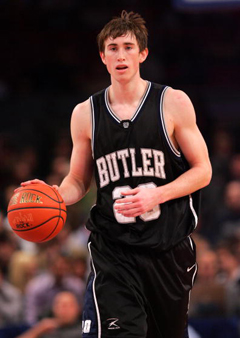
\includegraphics[height = .8\textheight]{C:/Users/Paul/Documents/STAT539Project/hayward}
	\end{figure}
\end{multicols}
	
	\end{frame}

\begin{frame}{Research Questions}
\begin{enumerate}
	\item %1
	Which factors are most important in helping a home team win a game?
	\item %2
	Do the effects of each covariate on the probability of winning change in games that go to overtime?
\end{enumerate}
	
\end{frame}

	
\section{Data}
\begin{frame}{The Data}
	Data are obtained from Kaggle.com's repository for the 2016 March Machine Learning Mania competition. Most of the people competing in this used predictive algorithms like random forests, etc. to predict outcomes. There were 
		\\
		\begin{itemize}
			\item Number of schools, etc.  
			\item \textbf{Predictors}:  
			
		\end{itemize}
	
\end{frame}

\begin{frame}{Variables}



\end{frame}

\begin{frame}{Prediction and Inference} 
Although the model is designed for inference, we believe that a good model ought to be able to predict outcomes with a reasonable degree of accuracy. We split the data into 70-30 training-test sets. 
\begin{figure}[r]
	
\includegraphics[height = .5\textheight]{C:/Users/Paul/Documents/STAT539Project/fakelebron}
\end{figure}
\end{frame}

	
	\section{Methods}
	
	\begin{frame}{Logistic Regression}
	Since the response is binary, we chose to fit a model with the \textbf{logit} link. We picked the logit link function for several reasons: 
	\begin{itemize}
		\item Logit - link allows for interpretation on probability scale
		\item It did not make sense to model game outcomes on a latent variable scale
		\item 		
	\end{itemize}
	\end{frame}
	

	
	
\begin{frame}{Model Space}
AIC comparisons etc. 
\end{frame}
	
	
\section{Results}

	\begin{frame}{The Model}
\begin{itemize}
	\item Estimates from the final model 
	\item goodness of fit
\end{itemize}	
\end{frame}	

	
	
\begin{frame}{Answering Research Questions}

\end{frame}	

\begin{frame}{Checking Prediction}
Secondary goal of the analysis. 
\end{frame}

\begin{frame}{Discussion}
Final thoughts and further work

\end{frame}

\begin{frame}
references
\end{frame}
	
	
\end{document}
